% DATE 6-page variant — trimmed copy of sections/05_experiments.tex
\section{Experimental Results}\label{sec:experiments}

\subsection{Setup}\label{sec:setup}

We evaluated on all seven benchmarks of the ICCAD 2024 CAD Contest Problem~B~\cite{yang2024contest,fang2024overview}: three released and four hidden cases, spanning millions of instances and weight profiles that price timing, power, area, and density very differently. All reported scores come from the official preliminary evaluator run on the final solution file, and every solution passed the evaluator's legality check plus the contest sanity and placement checkers. The flow is implemented in C++ with OpenMP on top of the strengthened open-source front end~\cite{baselineRepo} described in Section~\ref{sec:background}; all refinement deltas below are measured against that strengthened base, not the stock public flow.

All results use a single unified configuration: one environment recipe, zero per-case hyperparameters, fixed by no-regression sweeps over the same seven cases. Like all published results on this benchmark it is selected in-sample; unlike them, no knob differs between cases, and it beat every per-case-tuned configuration this flow had previously produced. We will release the seven solution files so every score is independently checkable. Experiments ran on a dual Intel Xeon E5-2630~v4 server (2.2\,GHz) using 8 threads. Because every operator runs to its convergence fixpoint rather than to a wall-clock cut, results are reproducible: six of the seven cases produce byte-identical solutions across all three repeats; on Hidden~4 one accept at floating-point noise flips between repeats, moving the final score by $2{\times}10^{-4}$\,\% (std/mean).

\subsection{Main Results}\label{sec:mainresults}

Table~\ref{tab:main} compares against every evaluator-comparable published result: the contest top-3 per-case costs, LBR (the contest winner's two-page late-breaking result~\cite{li2025lbr}, self-reported average ratio 0.988 against first place), and the DATE~2026 flow~\cite{chen2026agile} (self-reported $0.2\%$ better than LBR). Under one unified baseline, ours is the only method that beats the top-3 best on every case, and it also beats \emph{both} published methods head to head on all seven cases: by $2.0\%$ on Case~2 and $20.9\%$ on Hidden~2 against LBR, and by $4.3\%$ and $12.3\%$ against the DATE~2026 flow. Hidden~2's outsized margin is itself mechanistic: on this power-dominated case, proxy-priced flows leave $2{\times}2\mathrm{b}{\to}4\mathrm{b}$ merges unexploited that exact pricing captures safely. TIMBER~\cite{dassarma2026timber} also reports on these cases, but under its own min--max normalization against a baseline re-run whose bin-violation counts differ from the official contest standings, so its scores cannot be placed in this table.

\begin{table*}[t]
\centering
\caption{Official evaluator scores on all seven Problem~B cases (lower is better). Top-3 costs as re-evaluated in~\cite{chen2026agile}; LBR as published (four significant digits)~\cite{li2025lbr}. Composites are average per-case ratios against the same top-3-best baseline for all methods. Where the two published baselines differ we use the stricter, making our margins conservative.}
\label{tab:main}
\small
\begin{tabular}{@{}lrrrrrr@{}}
\toprule
Case & Top-3 best & LBR~\cite{li2025lbr} & DATE'26~\cite{chen2026agile} & Ours & $\Delta$ vs top-3 & T (s) \\
\midrule
Case 1   & 739{,}235{,}861 & 738{,}800{,}000 & 736{,}602{,}486 & \textbf{734{,}766{,}838} & $-0.60\%$ & 199 \\
Case 2   & 744{,}231       & 738{,}400       & 756{,}559       & \textbf{723{,}780}       & $-2.75\%$ & 1{,}216 \\
Case 3   & 727{,}971{,}140 & 728{,}800{,}000 & 727{,}757{,}372 & \textbf{726{,}236{,}872} & $-0.24\%$ & 2{,}582 \\
Hidden 1 & 31{,}507{,}917  & 31{,}270{,}000  & 30{,}946{,}401  & \textbf{30{,}199{,}301}  & $-4.15\%$ & 203 \\
Hidden 2 & 13{,}408{,}414  & 12{,}760{,}000  & 11{,}510{,}067  & \textbf{10{,}097{,}053}  & $-24.70\%$ & 2{,}202 \\
Hidden 3 & 55{,}941{,}500  & 55{,}920{,}000  & 55{,}973{,}041  & \textbf{55{,}789{,}826}  & $-0.27\%$ & 1{,}787 \\
Hidden 4 & 728{,}497{,}353 & 726{,}900{,}000 & 727{,}798{,}594 & \textbf{726{,}154{,}906} & $-0.32\%$ & 2{,}619 \\
\midrule
Composite & 1.000 & 0.991 & 0.979 & \textbf{0.953} & & \\
\bottomrule
\end{tabular}
\end{table*}

\subsection{Ablation}\label{sec:ablation}

Table~\ref{tab:ablation} isolates each contribution by enabling the operators cumulatively on the three most cost-sensitive cases; the base row is the strengthened proxy-priced front end of Section~\ref{sec:background} with the entire refinement layer disabled, so the deltas attribute to refinement only. Exact batch re-pairing is the largest single lever everywhere ($-2.7\%$ to $-8.6\%$). Repairing the inherited move-space exclusion (an audit finding rather than an algorithmic contribution) and structural rebanking pay on the two cases whose residual cost sits in banking structure (Case~2, Hidden~2), with rebanking alone worth $-1.4\%$ and $-2.5\%$ respectively. Density pricing acts exactly where overfilled bins exist: it moves Hidden~1 by $-0.4\%$ and is a verified no-op on Case~2 and Hidden~2, whose bin counts are already legal. No stage regresses any case.

A controlled counterfactual isolates pricing itself: rerunning the full flow with the rebanking operator unchanged except that each accept is quoted by the inherited one-hop proxy (identical candidates, staging, and surrounding operators) degrades every case --- $+0.15\%$ on Case~2, $+0.90\%$ on Hidden~1, $+0.41\%$ on Hidden~2. Two observations follow. Exact pricing wins uniformly even inside an otherwise identical architecture; and the staged, monotone commit structure independently contains the damage that historically compounded when proxy pricing drove in-flow merging (Sec.~\ref{sec:background}). Pricing fidelity and commit architecture are separable safeguards, and the historical cascades required losing both.

\begin{table}[t]
\centering
\caption{Cumulative ablation, official evaluator score (lower is better).}
\label{tab:ablation}
\small
\begin{tabular}{@{}lrrr@{}}
\toprule
Configuration & Case 2 & Hidden 1 & Hidden 2 \\
\midrule
Front end (no refinement)       & 761{,}159 & 30{,}615{,}486 & 11{,}614{,}120 \\
$+$ exact batch re-pairing      & 740{,}251 & 30{,}336{,}791 & 10{,}619{,}091 \\
$+$ move-space repair           & 733{,}903 & 30{,}335{,}019 & 10{,}356{,}851 \\
$+$ structural rebanking        & 723{,}780 & 30{,}327{,}025 & 10{,}097{,}053 \\
$+$ density-term pricing        & 723{,}780 & 30{,}199{,}301 & 10{,}097{,}053 \\
\bottomrule
\end{tabular}
\end{table}

\subsection{Anytime Behavior and Runtime}\label{sec:anytime}\label{sec:runtime}

Figure~\ref{fig:anytime} plots the official evaluator score, measured by running the evaluator binary on solutions dumped at every stage boundary, against refinement wall-clock on the two cases with the largest headroom. The descent is monotone across all 63 checkpoints on all seven cases.

\begin{figure}[t]
\centering
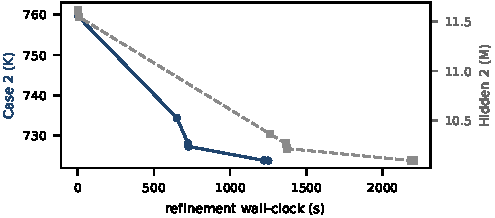
\includegraphics[width=0.85\linewidth]{figs/anytime.pdf}
\caption{Official evaluator score vs.\ refinement wall-clock, from evaluator runs on stage-boundary dumps; Case~2 (left axis, solid), Hidden~2 (right axis, dashed).}
\label{fig:anytime}
\end{figure}

Per-case wall times appear in Table~\ref{tab:main}. Convergence early-exit adapts effort automatically; the suite completes in about three hours on one server, bit re-pairing dominating the budget (66--96\% of refinement time). Because the framework is anytime, the runtime--quality trade can be quoted at any budget: capping refinement to a 1--2.5 minute class yields composite 0.966, a 3--8 minute class 0.958, and full convergence 0.953; every point on that curve beats the best published composite (0.979). The base flow itself completes in 21--36\,s, comparable to the contest entries; the budget beyond that is spent evaluating millions of exactly-priced moves that faster flows never attempt. For reference, the DATE~2026 flow finishes each case in about three seconds at composite 0.979~\cite{chen2026agile}, LBR spends up to 77\,s at 0.991~\cite{li2025lbr}, and we spend minutes per case on an older 2.2\,GHz server to reach 0.953.
